% Conformal Prediction Method Comparison
% Replaces: tab:conformal-comparison in section_conformal_empirical_validation.tex
% Scatter/bubble chart showing coverage vs interval width tradeoff

\begin{figure}[htbp]
\centering
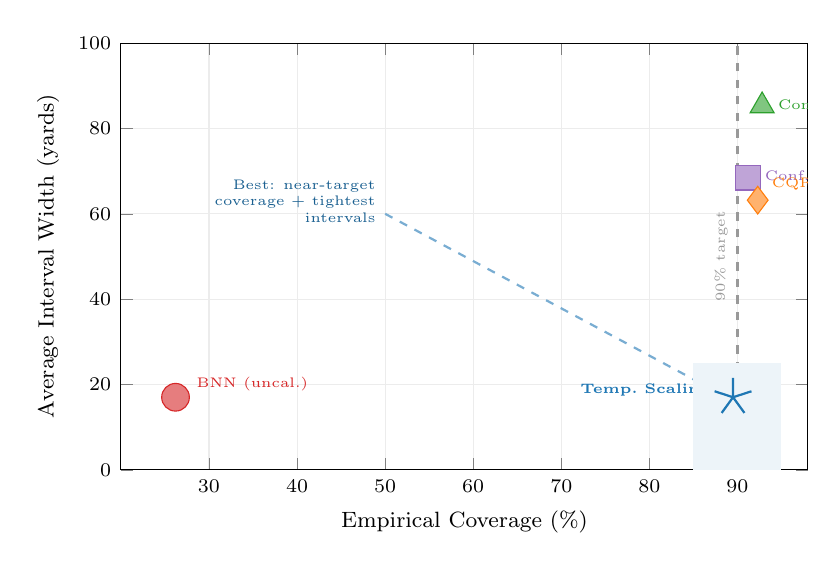
\begin{tikzpicture}
\definecolor{colBNN}{RGB}{214,39,40}
\definecolor{colTemp}{RGB}{31,119,180}
\definecolor{colConfBNN}{RGB}{148,103,189}
\definecolor{colConfRF}{RGB}{44,160,44}
\definecolor{colCQR}{RGB}{255,127,14}

\begin{axis}[
  width=0.85\textwidth,
  height=7cm,
  xlabel={Empirical Coverage (\%)},
  xlabel style={font=\footnotesize},
  ylabel={Average Interval Width (yards)},
  ylabel style={font=\footnotesize},
  xmin=20, xmax=98,
  ymin=0, ymax=100,
  xtick={30,40,50,60,70,80,90},
  xticklabel style={font=\scriptsize},
  yticklabel style={font=\scriptsize},
  grid=major,
  grid style={gray!15},
]

% Target coverage line
\draw[black!40, dashed, thick] (axis cs:90,0) -- (axis cs:90,100);
\node[font=\tiny, text=black!40, anchor=south, rotate=90] at (axis cs:90,50) {90\% target};

% BNN Baseline (uncalibrated) — large red marker
\addplot[only marks, mark=*, mark size=5pt, colBNN, fill=colBNN!60]
  coordinates {(26.2, 17.0)};
\node[font=\tiny, anchor=west, text=colBNN] at (axis cs:27.5,20) {BNN (uncal.)};

% Temperature Scaling — large blue star (winner)
\addplot[only marks, mark=star, mark size=7pt, colTemp, fill=colTemp!60, thick]
  coordinates {(89.5, 17.0)};
\node[font=\tiny\bfseries, anchor=south east, text=colTemp] at (axis cs:88,15) {Temp.\ Scaling};

% Split Conformal (BNN) — purple
\addplot[only marks, mark=square*, mark size=4.5pt, colConfBNN, fill=colConfBNN!60]
  coordinates {(91.2, 68.5)};
\node[font=\tiny, anchor=west, text=colConfBNN] at (axis cs:92,68.5) {Conf.\ (BNN)};

% Split Conformal (RF) — green
\addplot[only marks, mark=triangle*, mark size=5pt, colConfRF, fill=colConfRF!60]
  coordinates {(92.8, 85.3)};
\node[font=\tiny, anchor=west, text=colConfRF] at (axis cs:93.5,85.3) {Conf.\ (RF)};

% CQR — orange
\addplot[only marks, mark=diamond*, mark size=5pt, colCQR, fill=colCQR!60]
  coordinates {(92.3, 63.2)};
\node[font=\tiny, anchor=south west, text=colCQR] at (axis cs:92.8,63.2) {CQR};

% Arrow showing temp scaling dominance
\draw[->, thick, colTemp!60, dashed] (axis cs:50,60) -- (axis cs:87,19);
\node[font=\tiny, text=colTemp!80!black, anchor=east, align=right] at (axis cs:50,63)
  {Best: near-target\\coverage + tightest\\intervals};

% Shade the ideal region
\fill[colTemp!8] (axis cs:85,0) rectangle (axis cs:95,25);

\end{axis}
\end{tikzpicture}
\caption[Conformal prediction method comparison]{Coverage vs.\ interval width for uncertainty quantification methods (2024 holdout). Temperature scaling (blue star) achieves near-optimal coverage (89.5\%) with the narrowest intervals (17.0 yards)---3.7$\times$ sharper than the best conformal method (CQR, 63.2 yards). Conformal methods guarantee $\geq 90\%$ coverage but at significant width cost. The shaded region marks the ideal operating point.}
\label{fig:conformal-comparison-chart}
\end{figure}
